\documentclass[12pt]{article}
\usepackage[a4paper,margin=1in]{geometry}
\usepackage{amsmath, amssymb}
\usepackage{graphicx}
\usepackage{hyperref}
\usepackage{fancyhdr}
\usepackage{enumitem}
\usepackage{titlesec}
\usepackage{tcolorbox}
\usepackage{color}
\usepackage{multicol}
\usepackage{parskip}
\usepackage{mdframed}
\usepackage{lipsum}
\usepackage{tikz}
\usepackage{quoting}
\usepackage{float}
\quotingsetup{vskip=0pt}

\newenvironment{pullquote}
  {\begin{quoting}[leftmargin=2em,rightmargin=2em]\itshape}
  {\end{quoting}}

\title{Fluid Organisation 2.0: A Flywheel of Flow}
\author{Marc-Daniel Ortega}
\date{June 5, 2025}

\pagestyle{fancy}
\fancyhf{}
\lhead{Marc-Daniel Ortega}
\rhead{Fluid Organisation 2.0}
\setlength{\headheight}{14.5pt}
\addtolength{\topmargin}{-2.5pt}
\rfoot{\thepage}

\begin{document}

\maketitle
\tableofcontents
\newpage

% Callout quote after Introduction

\section{Introduction: The Problem Is Not Speed—It Is Systemic Mismatch}

In pursuit of agility, most organisations impose a single cadence across all teams. This uniformity may appear efficient, yet it conceals profound structural dysfunction. Core teams—responsible for platform stability, security, and compliance—are expected to accelerate on demand. Surface teams—those closest to market signals—lack the feedback loops and tooling required to act responsibly at pace. Governance is exercised by exception. Platforms struggle for adoption. Product teams repeatedly reinvent solutions. When failures occur, blame is misdirected.

This is not a failure of individuals. It is a failure of organisational design.

Nature demonstrates alternative models. In tectonics, movement at the surface is driven by slow, circulating energy deep within the mantle. In hydrodynamics, velocity varies smoothly across a pipe or river—layered, not uniform. In machinery, gearboxes facilitate motion not by enforcing speed, but by adapting torque and transmission to context.

A \textit{fluid organisation} learns from these systems. It recognises that speed without structure results in turbulence, and that layers of motion can coexist if connected by appropriate mechanisms. Signal is not merely information; it is the precondition for adaptation.

The Fluid Organisation draws inspiration from the systems thinking tradition established by \textbf{Donella Meadows}. As Meadows taught, effective systems are not controlled—they are understood, shaped, and evolved through feedback, structure, and clarity of purpose. The aim is not to accelerate blindly, but to observe, diagnose, and intervene with precision. Organisations are viewed not as machines to optimise, but as \textbf{dynamic systems to read, steer, and mature}.

\begin{pullquote}
Signal is not information. It is the precondition for adaptation.
\end{pullquote}

Through this lens, it becomes apparent:
\begin{itemize}
    \item Reusable capability is fostered, not mandated.
    \item Experimentation becomes input to architecture.
    \item Platform teams operate as flywheels, not helpdesks.
    \item Leadership aligns motion through rhythm rather than rigidity.
\end{itemize}

The promise of the Fluid Organisation is not speed or control, but \textbf{engineered coherence}.

\section{The Layered Model and Flywheel Mechanics}

The Fluid Organisation operates across three primary strata: the \textbf{Core}, the \textbf{Surface}, and the \textbf{Flywheel}. Each layer exhibits a distinct motion profile, analogous to natural and mechanical systems. Together, they form a dynamic structure in which feedback and adaptation replace rigidity and command.

\begin{figure}[H]
  \centering
  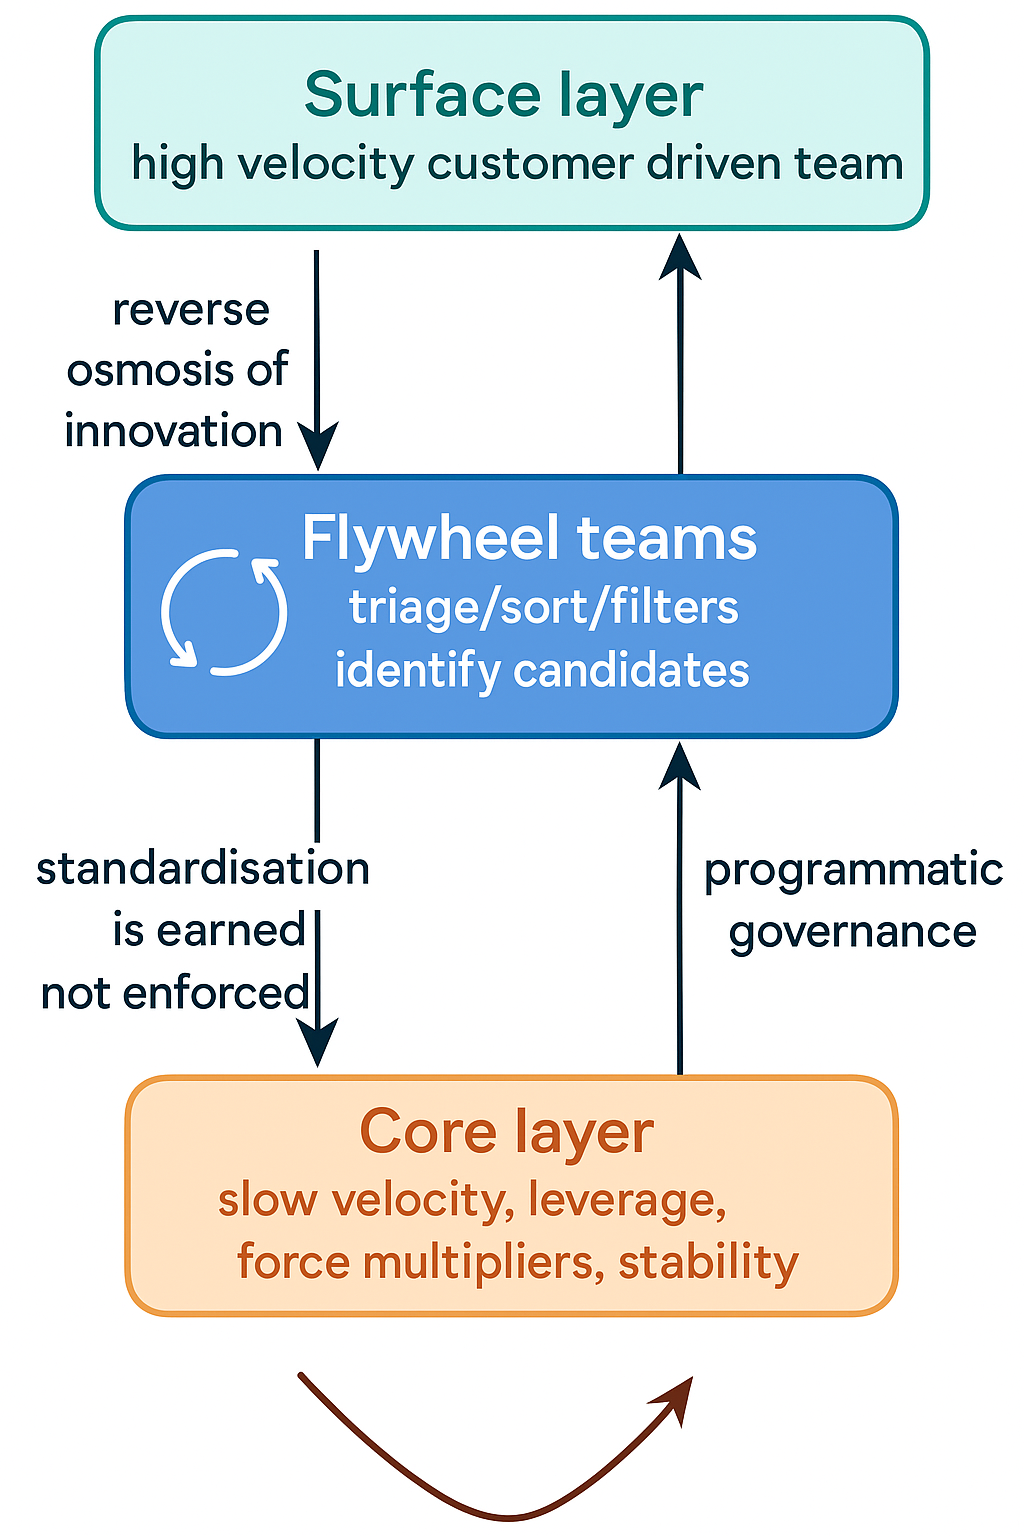
\includegraphics[width=0.8\textwidth]{images/org.png}
  \caption{Layered Flywheel Structure: Core \textrightarrow{} Flywheel \textrightarrow{} Surface}
\end{figure}

\subsection*{The Core Layer}

The Core comprises durable, capability-rich teams responsible for shared infrastructure, security, compliance, and internal platforms. Their work demonstrates low tolerance for rework, high standards for stability, and long time horizons.

Motion in the Core is \textit{deliberate} rather than reactive. It is akin to tectonic plates—slow, steady, yet powerful. The Core maintains the integrity of shared standards and provides reusable primitives that support broader organisational flow. It does not pursue trends; it absorbs validated outcomes.

\subsection*{The Surface Layer}

The Surface layer consists of product, experimentation, and customer-facing teams. These teams operate close to real-world signals such as market changes, user feedback, and competitive dynamics.

Motion in the Surface is \textit{fast, iterative, and explorative}. It is comparable to a swift-moving river: responsive and adaptive, but susceptible to turbulence without clear boundaries. Surface teams generate ideas, test assumptions, and respond quickly to stimuli.

\subsection*{The Flywheel Layer}

Situated between Core and Surface is the \textbf{Flywheel}. This is not a team, but a transductive function. It converts speed into structure and structure into opportunity.

The Flywheel enables layered motion by ensuring that:
\begin{itemize}
    \item Surface innovations are triaged, metabolised, and, when appropriate, standardised.
    \item Core constraints are articulated as high-quality, discoverable interfaces.
    \item Feedback loops are closed across layers through metrics, tooling, and governance patterns.
\end{itemize}

The Flywheel acts as a continuously variable transmission. It does not enforce fixed rhythms or cadences; instead, it modulates motion, enabling \textit{fluid synchronisation} without demanding uniformity.

In this model, coherence is maintained not by slowing all teams, but by ensuring each layer moves according to its nature—connected through \textbf{dynamic interfaces and transductive feedback}.

Where traditional models attempt to eliminate variance, the Fluid Organisation seeks to \textit{channel} it.


\section{Core Metrics and Mental Models}

The original white paper introduced metrics employing hydrodynamic analogues—\textbf{Org Re} (Organisational Reynolds Number) and \textbf{Shear Index}—to measure turbulence and misalignment in delivery systems. In version 2.0, this approach is retained and expanded with additional metrics: \textbf{TQS} (Transduction Quality Score) and \textbf{Entropic Pressure}.

These metrics reflect a shared philosophy: \textit{coherence is not the absence of change, but the presence of structured motion}. Each metric captures an aspect of system behaviour:
\begin{itemize}
    \item Org Re measures delivery speed relative to interface maturity (friction).
    \item TQS tracks signal integrity across time and layers.
    \item Entropic Pressure quantifies systemic decay and misalignment.
\end{itemize}

\subsection{Org Re: Organisational Reynolds Number}

\textbf{Formula:}
\[
\text{Org Re} = \frac{\text{Deployments} \times \text{Active Teams}}{\text{Interface Maturity Index}}
\]

\textbf{Philosophy:} Derived from the Reynolds Number in fluid dynamics, Org Re identifies when structured delivery yields to chaotic motion due to underdeveloped interfaces.

\textbf{Component Details:}
\begin{itemize}
    \item Deployments: Number of production releases within a defined time window.
    \item Active Teams: Teams contributing to those releases.
    \item Interface Maturity Index (IMI): Composite score from 1–5 based on documentation, onboarding, governance, and support maturity.
\end{itemize}

\textbf{Interpretation Bands:}
\begin{itemize}
    \item $<$ 100: Delivery is stable relative to structure.
    \item 100--200: Friction is emerging; Flywheel reinforcement is advisable.
    \item $>$ 200: Systemic turbulence; restructure or pause delivery.
\end{itemize}

\subsection{TQS: Transduction Quality Score}

\textbf{Formula:}
\[
\text{TQS} = \frac{\text{Signal Traceability} \times \text{Interface Impact}}{\text{Time to Actionable Outcome}}
\]

\textbf{Philosophy:} TQS measures how effectively the organisation transduces intent into value.

\textbf{Component Details:}
\begin{itemize}
    \item Signal Traceability (1–5): Whether the origin of the idea can be traced to implementation.
    \item Interface Impact (1–5): Whether the signal influenced a durable interface or shared capability.
    \item Time to Actionable Outcome: Days from request to usable output.
\end{itemize}

\textbf{Interpretation:}
\begin{itemize}
    \item High TQS ($>$ 2.5): Strong signal propagation and Flywheel coherence.
    \item Low TQS ($<$ 1.5): Noise, reactivity, or signal bypass.
\end{itemize}

\subsection{Entropic Pressure}

\textbf{Formula:}
\[
\text{EP} = \frac{\text{Redundancy} \times \text{Drift} \times \text{Rework}}{\text{Adoption Rate}}
\]

\textbf{Philosophy:} Entropic Pressure captures how much energy is lost to duplication, divergence, or abandonment.

\textbf{Component Details:}
\begin{itemize}
    \item Redundancy: Count of duplicated solutions.
    \item Drift: Divergent or unmaintained forks.
    \item Rework: Duplicated or restarted initiatives.
    \item Adoption Rate: Percentage of surfaced interfaces adopted within the target time frame.
\end{itemize}

\textbf{Interpretation:}
\begin{itemize}
    \item High EP: Systemic decay and convergence failure.
    \item Low EP: Structural clarity and reuse are dominant.
\end{itemize}

\subsection{Exploratory Metrics}
\begin{itemize}
    \item Feedback Latency Index (FLI)
    \item Alignment Drift Score (ADS)
    \item Reuse Drag Index (RDI)
    \item Interface Density Index (IDI)
    \item Flow Misalignment Score (FMS)
\end{itemize}

These metrics are emerging and require calibration, but they help surface systemic inefficiencies and signal loss.

\section{Interface Maturity and Enablement}

Interfaces are the essential transmission points in a Fluid Organisation. They are not only APIs or technical surfaces; they are contracts between layers. They define how capabilities are discovered, reused, and evolved. When designed well, they reduce friction. When neglected, they become bottlenecks, sources of duplication, or points of entropy.

\subsection*{Interface Maturity Index (IMI)}

The Interface Maturity Index (IMI), first introduced in Org Re, offers a structured scoring system for interface quality across five dimensions:
\begin{itemize}
    \item \textbf{Discoverability}: Is the interface visible and well documented?
    \item \textbf{Onboarding}: Are paved paths or examples available for first use?
    \item \textbf{Change Governance}: Are versioning and deprecation policies clear?
    \item \textbf{Self-service Capability}: Can teams adopt without meetings or manual intervention?
    \item \textbf{Feedback Mechanisms}: Are there channels for feedback and improvement?
\end{itemize}

\textbf{Score bands:}
\begin{itemize}
    \item 1--2: Informal, undocumented, internal only
    \item 3: Controlled adoption with some guidance
    \item 4: Productised with cross-team reuse
    \item 5: Integrated across domains with metrics and support
\end{itemize}

\subsection*{Primary vs. Secondary Enablement}

Enablement converts capability into adoption. We distinguish between:
\begin{itemize}
    \item \textbf{Primary Enablement}: Builders and maintainers of interfaces.
    \item \textbf{Secondary Enablement}: Practices that support signal flow, e.g., triage clinics, reuse showcases, etc.
\end{itemize}

Together, they shape the interface layer of the Flywheel.

\subsection*{Patterns of Effective Enablement}
\begin{itemize}
    \item \textbf{Interfaces as Products}: Ownership, support, and roadmaps.
    \item \textbf{Self-Service by Default}: Minimal friction for adoption.
    \item \textbf{Paved Paths and Templates}: Ready-to-use examples.
    \item \textbf{Governance by Design}: Constraints embedded into workflows.
    \item \textbf{Adoption Metrics}: Track real usage, not just existence.
\end{itemize}

\subsection*{Anti-patterns}
\begin{itemize}
    \item \textbf{Gatekeeping}: Rigid approvals that delay progress.
    \item \textbf{Shadow Documentation}: Outdated, hidden, or siloed knowledge.
    \item \textbf{Tool Pushing}: Enforced tools without context or support.
    \item \textbf{One-off Integrations}: Quick fixes that bypass shared layers.
    \item \textbf{Reinvention Loops}: Duplicate capabilities due to poor visibility.
\end{itemize}

Each of these erodes Org Re, reduces TQS, and raises Entropic Pressure.

\section{The Flywheel Layer in Practice}

The Flywheel is the least visible yet most vital component of the Fluid Organisation. It connects the layered motions of Core and Surface not through hierarchy, but through continuous transduction---transforming signals, packaging knowledge, and modulating flow.

Unlike traditional structures, the Flywheel does not enforce coordination through planning. It creates coherence through feedback. It does not control teams---it converts speed into structure and structure into opportunity.

\subsection*{The Nature of Flywheel Motion}

The Flywheel behaves like a continuously variable transmission (CVT). It translates fast signals from the Surface into stable capabilities for the Core---and vice versa. Its role is to absorb misalignment, metabolise patterns, and restore flow.

When functioning well, it reduces:
\begin{itemize}
    \item Redundant local innovation
    \item Blocked reuse or slow onboarding
    \item Friction between product teams and platform layers
\end{itemize}

When absent, it results in:
\begin{itemize}
    \item Sprawl in interface design
    \item Duplication across product verticals
    \item Mistrust of shared capabilities
\end{itemize}

\subsection*{Five Flywheel Patterns That Restore Motion\\Without Chaos}

These patterns are repeatable strategies that restore transductive flow without centralised control.

\subsubsection*{1. Shadow Integrators}

Platform engineers or senior ICs embed temporarily in product teams. Their goal is to observe how local solutions emerge and then extract reusable elements for convergence. After one or two cycles, they exit, leaving paved paths or hardened templates.

\textbf{Use case:} Surfacing reuse candidates before abstraction

\textbf{Metric effect:} Boosts TQS, lowers redundancy (Entropic Pressure)

\subsubsection*{2. Signal Clinics}

Recurring, time-boxed sessions where teams pitch needs, share friction points, or surface emergent patterns. The Flywheel triages these signals for convergence, packaging, or deferral.

\textbf{Use case:} Continuous intake and feedback

\textbf{Metric effect:} Increases TQS by closing loops, stabilises Org Re

\subsubsection*{3. Pattern Shepherds}

Cross-cutting leaders who monitor how local innovations spread. They connect teams, harmonise naming and structure, and guide convergence into interfaces or practices.

\textbf{Use case:} Managing design divergence before it becomes entropy

\textbf{Metric effect:} Reduces drift, increases adoption rate

\subsubsection*{4. Reuse Jams}

Collaborative, themed events that challenge teams to solve real use cases using only shared primitives. Enables learning, surfaces gaps, and reinforces programmatic governance.

\textbf{Use case:} Teaching by doing

\textbf{Metric effect:} Elevates IMI scores, lowers Reuse Drag Index

\subsubsection*{5. Flow Cells}

Temporary, high-intensity convergence teams focused on a high-friction area. They stabilise interfaces, align producers and consumers, and dissolve once the domain flows smoothly.

\textbf{Use case:} Crisis-to-coherence \\
transformation

\textbf{Metric effect:} Rapidly reduces Entropic Pressure and Feedback Latency

\vspace{1em}
Each pattern is a practical instantiation of Flywheel logic: adaptive, transductive, and coherence-oriented.

\section{Patterns and Anti-patterns}

Where coherent Flywheel operations generate clarity and convergence, failed implementations amplify entropy. Anti-patterns are not simply mistakes; they are systemic regressions\\---local optimisations that erode global motion. They emerge when foundational principles of the Fluid Organisation are violated, often under pressure or misinterpretation.

\subsection*{6.1 Organisational Anti-patterns}

\begin{itemize}
    \item \textbf{Ticket Ops:} Platform teams treated as reactive support queues. The work surface becomes fragmented, feedback loops collapse, and enablement is replaced by backlog management.
    
    \item \textbf{Over-scaling the Core:} When every team declares itself platform, convergence stalls and responsibility dilutes. Redundant services emerge under the guise of specialisation.
    
    \item \textbf{Split Ownership of Intent and Execution:} Strategy is held separately from delivery. The “what” and “why” are specified upstream, and engineering is treated as downstream labour. This breaks feedback loops and damages TQS.
    
    \item \textbf{Ghost Governance:} Policies exist but are decoupled from interfaces. Developers navigate hidden contracts, and reuse declines due to ambiguity.
    
    \item \textbf{Symbolic Enablement:} Documentation exists, but interfaces are not discoverable. Office hours are held, but no follow-up occurs. Reuse metrics exist, but are not tracked.
\end{itemize}

\subsection*{6.2 Interface Anti-patterns}

\begin{itemize}
    \item \textbf{API Bloat:} Core systems expose interfaces designed for every use case, leading to complexity and confusion. Surface teams revert to duplicating logic.
    
    \item \textbf{Tightly Coupled Contracts:} Interfaces change too often or lack clear deprecation policies, raising rework incidence and Org Re.
    
    \item \textbf{Shadow Paving:} Teams create their own paved paths without alignment, \\
    diverging from the Flywheel’s convergence intent.
    
    \item \textbf{One-off Integrations:} Built under urgency, they resist absorption. The Flywheel becomes bypassed rather than reinforced.
\end{itemize}

\subsection*{6.3 Cultural Anti-patterns}

\begin{itemize}
    \item \textbf{Celebration of Local Heroics:} High-output teams are celebrated even when their solutions duplicate existing capabilities.
    
    \item \textbf{Mistrust of Shared Systems:} Perceived slowness in the Flywheel encourages local workarounds, bypassing convergence mechanisms.
    
    \item \textbf{Performative Agility:} Organisations speak of autonomy and speed, yet operate through over-specified roadmaps and structural control.
    
    \item \textbf{Governance as Policing:} Instead of enabling safe boundaries, governance arrives only as enforcement---often post-failure.
\end{itemize}

\subsection*{6.4 The Compound Effect}

Anti-patterns rarely operate in isolation. A split between strategy and implementation (structural) encourages ghost governance (interface), which enables shadow paving (practice), and reinforces performative agility (culture).

When the system exhibits:
\begin{itemize}
    \item High Org Re,
    \item Low TQS,
    \item Rising Entropic Pressure,
\end{itemize}
the source is often traceable to two or more anti-patterns converging.

The solution is not merely correction. It requires rebalancing flows, recommitting to feedback loops, and restoring the purpose of the Flywheel---not as a buffer, but as a system transducer.

\section{Systems Thinking and the Legacy of -- Donella Meadows}

The Fluid Organisation model is grounded in systems thinking. It does not merely describe motion—it examines \textit{why} certain motions persist, degrade, or harmonise. This perspective owes much to the work of \textbf{Donella Meadows}, whose insights into systemic purpose, feedback loops, delays, and leverage points frame how we approach organisational design.

\subsection*{7.1 Feedback Loops}

In Meadows’ terminology, feedback loops maintain the identity of the system. Reinforcing loops amplify motion. Balancing loops stabilise it. In the Fluid Organisation:
\begin{itemize}
    \item \textbf{TQS} is a diagnostic for feedback quality.
    \item \textbf{Signal Clinics} and \textbf{Packaging Sprints} close feedback gaps.
    \item The \textbf{Flywheel} manages the gradient between experimentation and consolidation.
\end{itemize}

Without designed feedback, systems stagnate or spiral. With healthy loops, coherence compounds.

\subsection*{7.2 Stocks, Flows, and Delays}

A \textit{stock} is a state; a \textit{flow} is the change of that state over time. \textbf{Delays} distort system response. Most platform failure modes stem from unacknowledged delay:
\begin{itemize}
    \item Surface teams move faster than the Core can absorb.
    \item Feedback arrives only after decay is visible.
    \item Adoption lags kill convergence momentum.
\end{itemize}

The Flywheel exists to mediate these flows. Metrics like \textbf{Entropic Pressure} and \textbf{Feedback Latency Index} make these dynamics visible.

\subsection*{7.3 System Purpose vs. Behaviour}

Meadows warned that “the least obvious part of the system, its function or purpose, is often the most crucial.”

In IT, organisations often adopt the \textit{language} of agility or enablement while structurally reinforcing silos, control, and output metrics. The system behaves differently than it claims.

The Fluid Organisation proposes a reversal:
\begin{itemize}
    \item Treat interfaces as \textbf{proof of coherence}, not policy.
    \item Let reuse and convergence be \textbf{observed}, not declared.
    \item Align feedback structures with the system’s \textbf{real purpose}: adaptability without chaos.
\end{itemize}

\subsection*{7.4 Leverage Points}

Meadows outlined places to intervene in a system. Among the most effective:
\begin{itemize}
    \item \textbf{Changing information flows}: What is visible, measurable, and understood.
    \item \textbf{Changing system rules}: What structures are enabled or forbidden.
    \item \textbf{Changing system goals}: What the system believes it is optimising.
\end{itemize}

The Fluid Organisation activates leverage points by:
\begin{itemize}
    \item Surfacing signal friction through \textbf{TQS} and \textbf{Org Re}.
    \item Encoding governance in \textbf{interfaces}, not documents.
    \item Shifting investment from tools to \textbf{enablement flywheels}.
\end{itemize}

This is not process improvement. It is \textbf{systemic leverage} in motion.

\section{Adoption Strategies and Vectors of Change}

The Fluid Organisation is not a framework to be rolled out. It is a way of seeing—and responding to—the organisation as a system in motion. Adoption begins not with structure, but with \textbf{perception}. The first shift is observational.

\subsection*{8.1 Start with the Metrics}

Measure before you intervene. Use \textbf{Org Re} to identify structural stress. Use \textbf{TQS} to detect signal decay. Use \textbf{Entropic Pressure} to surface systemic entropy. These are not performance metrics—they are \textit{feedback readers}.

\subsection*{8.2 Pilot a Single Flywheel Pattern}

Do not build a new department. Trial one Flywheel function:
\begin{itemize}
    \item Run a \textbf{Signal Clinic}.
    \item Embed a \textbf{Shadow Integrator}.
    \item Facilitate a \textbf{Reuse Jam}.
\end{itemize}

Small patterns, if successful, increase local coherence. That coherence is your next vector.

\subsection*{8.3 Treat Interfaces as Product}

If your team produces something meant for reuse, it must behave like a product:
\begin{itemize}
    \item It has an owner.
    \item It has telemetry.
    \item It improves through feedback.
\end{itemize}

Measure adoption. Build paved paths. Maintain clarity.

\subsection*{8.4 Align Incentives Around Systemic Outcomes}

Do not reward local speed alone. Reward reduction of \textbf{Org Re}. Recognise convergence. Track rising \textbf{TQS} as evidence of platform health. Celebrate high-leverage reuse.

\subsection*{8.5 Reframe Governance}

Governance in a Fluid Organisation is not gatekeeping. It is constraint embedded in \textbf{interface form}:
\begin{itemize}
    \item Validated schemas
    \item Auto-provisioned access
    \item Immutable defaults
\end{itemize}

Let systems guide behaviour, not after-the-fact enforcement.

\subsection*{8.6 Teach Mental Models, Not Playbooks}

You cannot copy another company’s Flywheel. But you can teach people how to recognise turbulence, signal decay, or enabling patterns. Share metaphors. Trace loops. Measure before acting.

The transition begins when teams see their organisation not as a roadmap to deliver, but as a system to observe and shape.

\begin{pullquote}
Signal is not information. It is the precondition for adaptation.
\end{pullquote}

\section{Conclusion: From Language to Leverage}

The Fluid Organisation is not a toolkit. It is a way of thinking, measuring, and acting in systems. It replaces the illusion of alignment with the engineering of coherence.

It does not promise speed—it enables sustainable motion. It does not centralise control—it distributes transduction. It does not avoid complexity—it metabolises it.

The metrics introduced—\textbf{Org Re}, \textbf{TQS}, and \textbf{Entropic Pressure}—do not judge teams. They reveal how systems respond to pressure, to signal, and to decay. The Flywheel does not enforce standards. It earns convergence by converting raw signal into reusable structure.

Adoption begins when you stop asking “\textit{How fast are we moving?}” and begin asking “\textit{What form is our motion taking—and what is it producing?}”

In the end, this model offers no certainty. But it does offer clarity:
\begin{itemize}
    \item Clarity of structure.
    \item Clarity of signal.
    \item Clarity of purpose.
\end{itemize}

That clarity becomes leverage.

This is what engineering becomes when it learns from rivers, from tectonics, from gearboxes—and from systems that endure not by force, but by form.

\newpage
\section*{Summary}

\addcontentsline{toc}{section}{Summary}

The Fluid Organisation 2.0 introduces a systems-based model of organisational motion and coherence. It moves away from rigid, uniform cadences and embraces layered dynamics across the Core, Surface, and Flywheel.

Rather than enforcing speed or control, it promotes structured adaptability, guided by signal flow and interface maturity. The Flywheel acts as a transductive engine, modulating energy between exploration and convergence, and supporting reuse without centralisation.

Three primary metrics—\textbf{Org Re}, \textbf{TQS}, and \textbf{Entropic Pressure}—allow organisations to monitor friction, feedback fidelity, and systemic decay.

Adoption is not procedural. It begins by observing what motion exists, restoring flow through flywheel patterns, and embedding coherence via enablement and governance by design. This model stands as a guide for those who want to build systems that endure, evolve, and converge without chaos.

\newpage
\section*{Glossary}

\addcontentsline{toc}{section}{Glossary}

\textbf{Org Re (Organisational Reynolds Number):} Measures delivery speed relative to interface maturity. Highlights turbulence from unmanaged scale or understructured delivery.

\textbf{TQS (Transduction Quality Score):} Assesses how effectively signals are translated into value-bearing outcomes. Tracks traceability, interface impact, and time to convergence.

\textbf{Entropic Pressure:} A measure of structural decay. Rises with duplication, drift, and rework. Falls with reuse, alignment, and stable adoption.

\textbf{Flywheel:} A layer that absorbs misalignment and transforms raw motion into structure and reuse. Bridges exploration and consolidation.

\textbf{IMI (Interface Maturity Index):} Composite score that evaluates discoverability, self-service, change governance, and feedback loops for reusable systems.

\begin{description}[style=nextline]
  \item[Signal Clinic] A lightweight, recurring triage session where teams surface friction, share insights, and coordinate flywheel feedback loops.
  \item[Flow Cell] A temporary, high-focus convergence team formed to resolve a high-friction domain, aligning producers and consumers.
  \item[Pattern Shepherd] A leadership role focused on guiding convergence of emergent design patterns across domains.
  \item[Shadow Integrator] A temporary embedded engineer who observes local patterns and extracts reusable components or paved paths.
\end{description}

\end{document}